\section{Introduction}
\begin{itemize}

\item There are many contemporary tools that provide the possibility 
to infer a phylogeny from genetic data (DNA, RNA, proteins). 
A popular Bayesian phylogenetic tool is called BEAST (\cite{beast}) 
and its cousin BEAST2 (\cite{beast2}).

\item BEAST is very flexible, providing the user with the option 
to set up all possible phylogenetic priors (e.g. site/clock/speciation model).

%Current limits in current tools.
\item However, currently available priors can be not suitable 
to analyze some specific datasets. 
With this work we aim to test whether or not 
the implementation of a new prior model 
is beneficial to study a specific kind of diversification process.

\item BEAST2 gives us the possibility to introduce new tree priors 
to infer phylogenies based on different assumptions 
on how the speciation process takes place.

\item One of such speciation processes is the multiple birth hypothesis,
a new model (described below) and thus currently absent in BEAST.

\item The Multiple birth hypothesis can be useful to explain a phenomenon 
that has always puzzled evolutionary biologists: 
what are the drivers of the diversification processes 
for those phylogenies that show an impressive amount of speciation events 
in relatively short times? 
The (constant-rate) birth-death (BD) model embodies the common assumption that 
only a single speciation event can occur at any given time.
The multiple-birth-death (MBD) model 
relaxes this assumption, allowing events in which 
large-scale environmental changes lead to a great number of species 
in relatively short time intervals. 
Such a hypothesis may be a better fit to describe the burst in systems 
like cichlid fish diversification in the 
African Great Lakes: Malawi, Tanganyika and Victoria 
(\cite{janzen2016}, \cite{janzen2017}).

\item However, it may be that current BD tree priors are good enough 
at detecting such events, with a (preferred) lower level of complexity. 
If this is the case one should always be more keen to adopt the simplest model.

\item Here we present our study with the aim of exploring 
when using a more complex MBD tree prior is warranted.
To do so, we simulate phylogenies using the MBD process, with
varying degrees of that process. To be explicit, we define
that degree, $s$, as the number of extinct and extant species created
during a co-occuring speciation event, 
$N_{\mathbb{M}}$, from the total number of extinct and extant species:

\begin{equation}
s = \frac{N_{\mathbb{M}}}{N_{\mathbb{M}} + N_{\mathbb{B}}}
\end{equation}


Here, $N_{\mathbb{B}}$ is the number of extinct and extant species created
during a default single-birth speciation event.

From such phylogenies with different degrees of $s$, we measure the
inference error we make today, would nature follow such a phylogeny.
The inference error we make today is caused by the assumption of a BD process
and by inherent noise in this inference. 

We have the hypothesis $\mathcal{H}_1$ that, for a higher $s$, 
the inference error $e$ will increase:

\begin{equation}
e = f(s)
\end{equation} 

Where $f$ is a monotonously increasing function of unknown shape.

\begin{figure}[!htbp]
  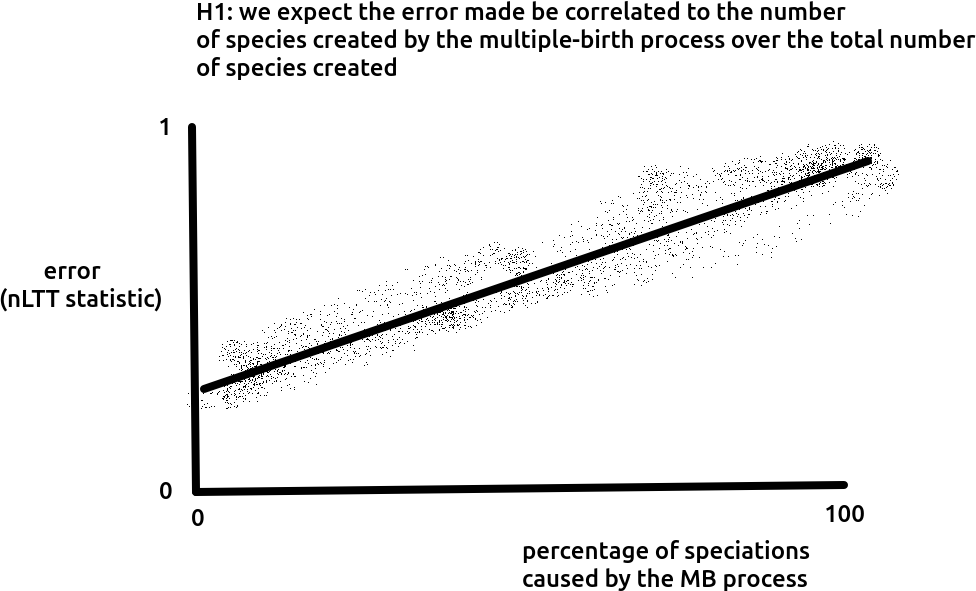
\includegraphics[width=\textwidth]{razzo-figures/fig_h_1.png}
  \caption{
    Hypothesis 1: we expect the error made be correlated to the number 
    of species created by the multiple-birth process over the total number 
    of species created
  }
  \label{fig:h_1}
\end{figure}

The MBD process has multiple components, that may cause 
different values of $e$ for identical values of $s$.

One MBD component that may cause 
different values of $e$ for identical values of $s$
is the MBD regime: which can be many modest 
multiple-speciation events, or few intense ones. 
As we have no prior expectations, we have the (null) hypothesis, 
$\mathcal{H}_0$, that the MBD regime has no effect on $e$.

\begin{figure}[!htbp]
  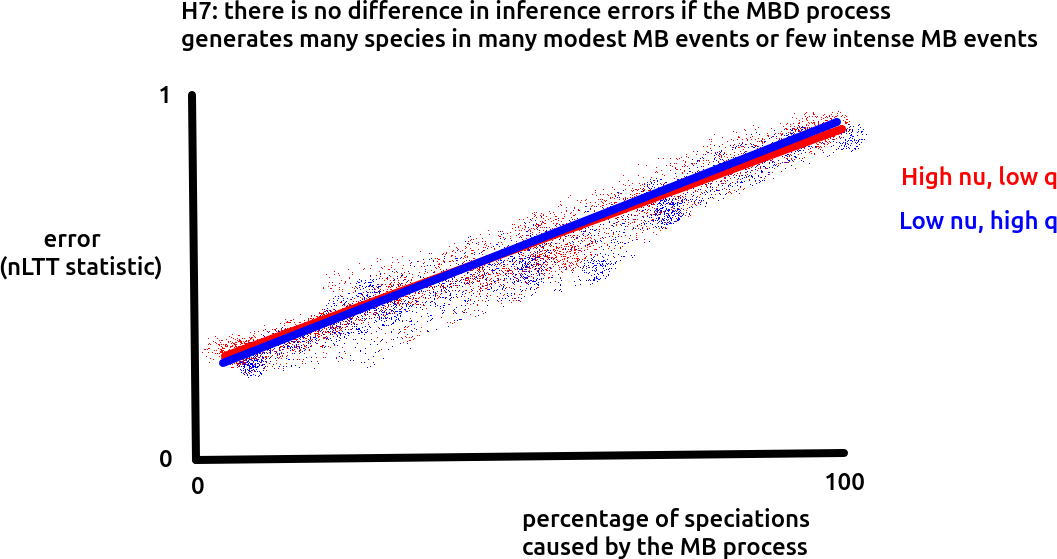
\includegraphics[width=\textwidth]{razzo-figures/fig_h_0.png}
  \caption{
    Hypothesis 0: there is no difference in inference errors if the MBD process
    generates many species in many modest MB events or few intense MB events
  }
  \label{fig:h_0}
\end{figure}

Another MBD component that may cause 
different values of $e$ for identical values of $s$
is the effect of extinction. 
As extinctions will hit lineages created by both speciation processes equally,
and we have no additionaly prior expectations,
we have the (null) hypothesis, 
$\mathcal{H}_2$, that extinction has no effect on $e$.

\begin{figure}[!htbp]
  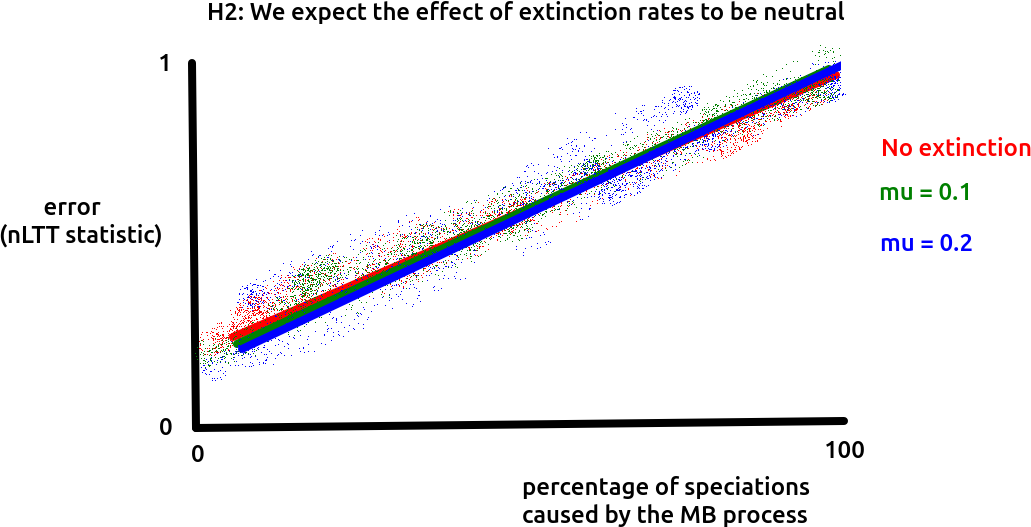
\includegraphics[width=\textwidth]{razzo-figures/fig_h_2.png}
  \caption{
    Hypothesis 2: the effect of extinction rates is neutral
  }
  \label{fig:h_2}
\end{figure}

Another MBD component that may cause 
different values of $e$ for identical values of $s$,
is the timing of a multiple-birth event: be it close to the
crown age or close to the present. 
Compared to a late multiple birth event, an early multiple birth event may have a 
longer-lasting effect (as the next speciation event will be later), but it
will create less new species, as there are still fewer taxa.
As we have no prior expectations,
we have the (null) hypothesis, 
$\mathcal{H}_3$, that the timing of multiple-birth events has no effect on $e$.

\begin{figure}[!htbp]
  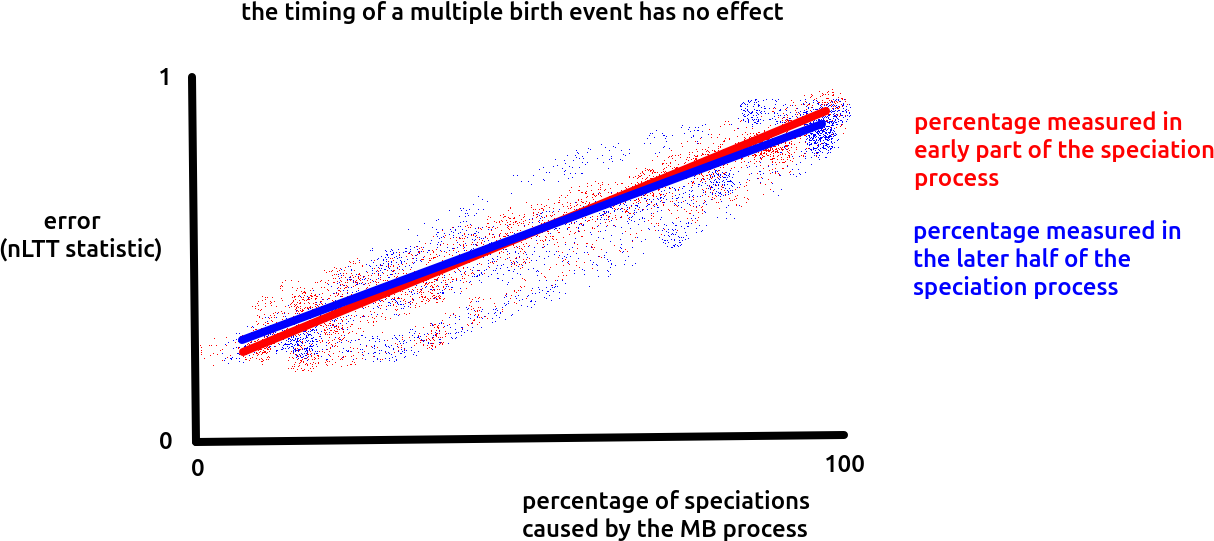
\includegraphics[width=\textwidth]{fig_h_3.png}
  \caption{
    Hypothesis 3: the timing of a multiple birth event has no effect.
  }
  \label{fig:h_3}
\end{figure}

Another MBD component that may cause 
different values of $e$ for identical values of $s$,
is the number of taxa in a phylogeny,
As there is no diversity dependency in any of the processes
and we have no further prior expectations, we have
the (null) hypothesis $\mathcal{H}_5$, that the number of
taxa has no effect on $e$.
As a higher number of taxa increases the information content in a
phylogeny, we have hypothesis $\mathcal{H}_6$ that the
variance in $e$ decreases.

\begin{figure}[!htbp]
  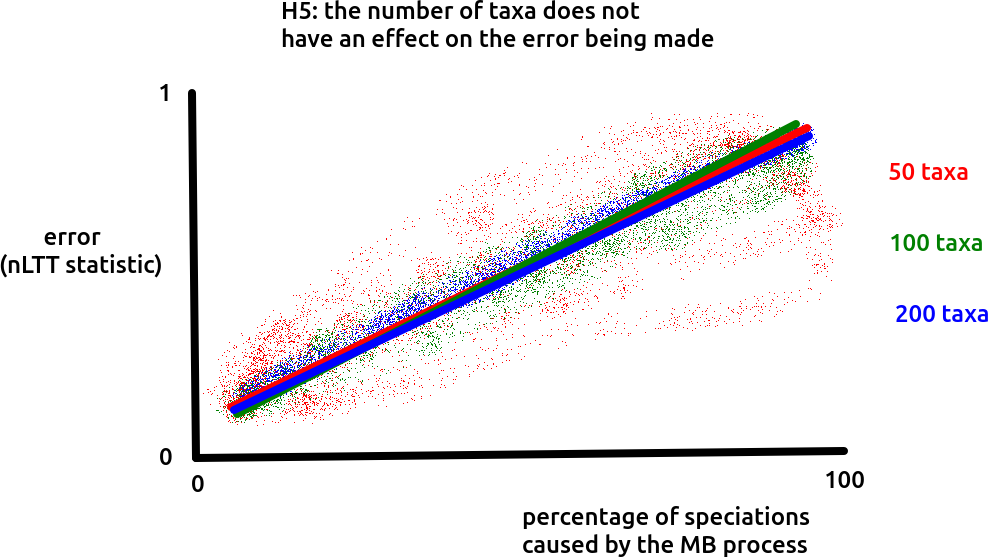
\includegraphics[width=\textwidth]{razzo-figures/fig_h_5.png}
  \caption{
    Hypothesis 5: the number of taxa does not
    have an effect on the error being made
  }
  \label{fig:h_5}
\end{figure}

\begin{figure}[!htbp]
  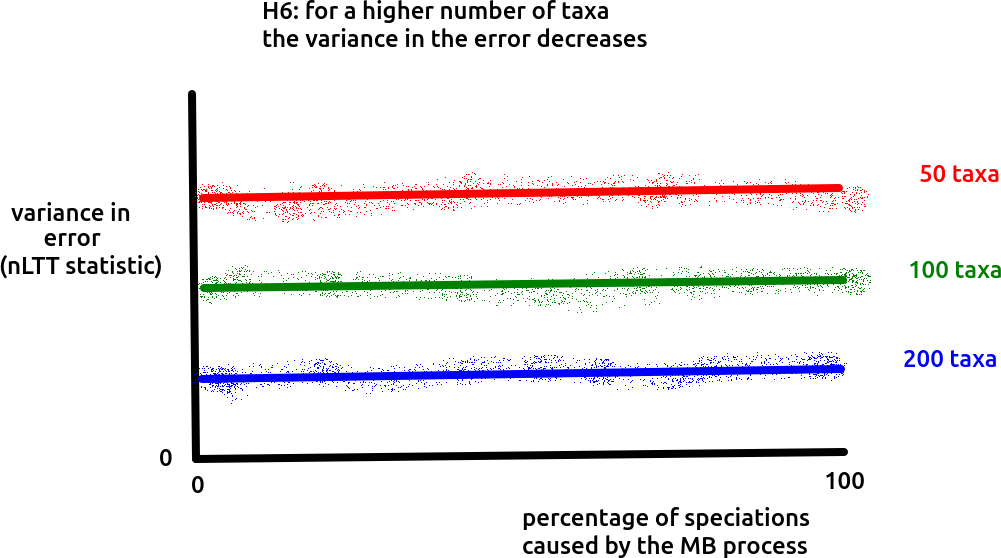
\includegraphics[width=\textwidth]{razzo-figures/fig_h_6.png}
  \caption{
    Hypothesis 6: for a higher number of taxa 
    the variance in the error decreases
  }
  \label{fig:h_6}
\end{figure}

\end{itemize}